\documentclass[epsfig,10pt,fullpage]{article}

\newcommand{\LabNum}{4}
\newcommand{\CommonDocsPath}{../../../../common/docs}
\addtolength{\textwidth}{1.5in}
\addtolength{\oddsidemargin}{-0.75in}
\addtolength{\topmargin}{-0.75in}
\addtolength{\textheight}{1.5in}
\addtolength{\evensidemargin}{0.75in}
\setlength\parindent{0pt}
\raggedbottom

\usepackage{ae,aecompl}
\usepackage{epsfig,float,times}
\usepackage[hypcap]{caption}
\usepackage[pdftex, colorlinks]{hyperref}
\usepackage{graphicx}
\usepackage[usenames, dvipsnames]{color}
\usepackage{rotating}
\usepackage{tikz}
\usetikzlibrary{automata,positioning}
\usepackage{placeins}

\widowpenalty 10000
\clubpenalty 10000

\newcommand{\red}[1]{{\color{red}\sf{#1}}}
\newcommand{\green}[1]{{\color{green}\sf{#1}}}
\newcommand{\blue}[1]{{\color{blue}\sf{#1}}}
\definecolor{PineGreen}{rgb}{0.0, 0.47, 0.44}
\definecolor{ForestGreen}{rgb}{0.13, 0.55, 0.13}
\definecolor{Brown}{rgb}{0.59, 0.29, 0.0}

\newcommand{\UPDatePublished}{Oct 2021}
\newcommand{\versnum}{21.1} %version number quartus/AMP
\newcommand{\quartusname}{Quartus\textsuperscript{\textregistered} Prime}	
\newcommand{\UPTextBar}{For \quartusname{} \versnum{}}
\newcommand{\thisyear}{2021 } %for copyright
\newcommand{\company}{FPGAcademy.org}
\newcommand{\longteamname}{FPGAcademy.org}
\newcommand{\teamname}{FPGAcademy}
\newcommand{\website}{FPGAcademy.org}

\newcommand{\productAcronym}{AMP}
\newcommand{\productNameShort}{Monitor Program}

\newcommand{\productNameMedTM}{A Monitor Program}
\newcommand{\productNameMed}{A Monitor Program}

%\newcommand{\headerLogoFilePath}[1]{#1/FPGAcademy.png}

% listings is a package that supports encapsulating source code in LaTeX conveniently
\usepackage{listings}

\def\expandparam\lstinputlisting[#1]#2{\edef\tmp{\noexpand\lstinputlisting[#1]{#2}}\tmp}

%%%%%%%%%%%%%%%%%%%% Source Code Formatting %%%%%%%%%%%%%%%%%%%%
\definecolor{globalCommentColour}{rgb}{0.588,0.588,0.588}

%%%%%%%%%%%%%%%%%%%%%%%%%%%%%%%%%%%%%%%%%%%%%%%%%%%%
% Defining language style
% NiosII ASM
\lstdefinelanguage[NiosII]{Assembler} {
  morekeywords={add, addi, and, andhi, andi, beq, bge, bgeu, bgt, bgtu, ble,  bleu, blt, bltu, bne, br, break,
  bret, call, callr, cmpeq, cmpeqi, cmpge, cmpgei, cmpgeu, cmpgeui, cmpgt, cmpgti, cmpgtu, cmpgtui, cmple,
  cmplei, cmpleu, cmpleui, cmplt, cmplti, cmpltu, cmpltui, cmpne, cmpnei, custom, div, divu, eret, flushd,
  flushda, flushi, flushp, initd, initda, initi, jmp, jmpi, ldb, ldbio, ldbu, ldbuio, ldh, ldhio, ldhu, ldhuio,
  ldw, ldwio, mov, movhi, movi, movia, movui, mul, muli, mulxss, mulxsu, mulxuu, nextpc, nop, nor, or, orhi, ori,
  rdctl, rdprs, ret, rol, roli, ror, sll, slli, sra, srai, srl, srli, stb, stbio, sth, sthio, stw, stwio,
  sub, subi, sync, trap, wrctl, wrtcl, wrprs, xor, xori, xorhi, xori},
  morekeywords=[2]{.abort, .ABORT, .align, .app-file, .ascii, .asciz, .balign, .byte, .comm, .data, .def,
  .desc, .dim, .double, .eject, .else, .end, .endef, .endif, .equ, .equiv, .err, .extern, .file, .fill, .float,
  .global, .globl, .hword, .ident, .if, .include, .int, .irp, .irpc, .lcomm, .lflags, .line, .linkonce, .ln,
  .list, .long, .macro, .mri, .nolist, .octa, .org, .p2align, .psize, .quad, .rept, .sbttl, .scl, .section,
  .set, .short, .single, .size, .sleb128, .skip, .space, .stadb, .stabn, .stabs, .string, .symver, .tag,
  .text, .title, .type, .val, .uleb128, .word},
  morekeywords=[3]{et, bt, gp, sp, fp, ea, sstatus, ra, pc, status, estatus, bstatus, ienable, ipending, cpuid,
  exception, pteaddr, tlbacc, tlbmisc, eccinj, badaddr, config, mpubase, mpuacc},
  sensitive=t,
  alsoletter=.,
  morestring=[b]",
  morecomment=[s]{/*}{*/},
  morecomment=[l]\#,
}[keywords,comments,strings]
   
%% NOTE: morekeywords=[2] are GNU directives.
   
\definecolor{niosInstructionColour}{rgb}{0.000,0.608,0.000}
\definecolor{niosDirectiveColour}{rgb}{0.000,0.000,0.902}
\definecolor{niosSpecialRegColour}{rgb}{0.000,0.000,0.000}
\definecolor{niosStringColour}{rgb}{0.808,0.482,0.000}
   
%% NOTE: To make bold use: =\bfseries\color{<colour>}
\lstdefinestyle{defaultNiosStyle} {
  language=[NiosII]{Assembler},
  stringstyle=\color{niosStringColour},
  keywordstyle=\color{niosInstructionColour},
  keywordstyle=[2]\color{niosDirectiveColour},
  keywordstyle=[3]\itshape\color{niosSpecialRegColour}
}
%%%%%%%%%%%%%%%%%%%%%%%%%%%%%%%%%%%%%%%%%%%%%%%%%%%%

%%%%%%%%%%%%%%%%%%%%%%%%%%%%%%%%%%%%%%%%%%%%%%%%%%%%
% Defining language style
% ArmA9 ASM
\lstdefinelanguage[ArmA9]{Assembler} {
  morekeywords={ADC, ADD, ADDS, AND, ANDS, B, BAL, BEQ, BGE, BGT, BL, BLT, BIC, BKPT, BLX, BNE, BX, CDP, CLZ, CMN, CMP, EOR,
  EORS, LDC, LDM, LDR, LDRB, LDRBT, LDRH, LDRSB, LDRSH, LDRT, LSL, MCR, MLA, MOV, MOVW, MOVT, MRC, MRS, MSR, MUL, MVN, ORR, PLD,
  ROR, RSB, RSC, SBC, SMLAL, SMULL, STC, STM, STR, STRB, STRBT, STRH, STRT, SUB, SUBS, SWI, SWP, SWPB, TEQ, UMLAL,
  PUSH, POP, MOVS, RORS, LSR},
  morekeywords=[2]{.abort, .ABORT, .align, .app-file, .ascii, .asciz, .balign, .byte, .comm, .data, .def,
  .desc, .dim, .double, .eject, .else, .end, .endef, .endif, .equ, .equiv, .err, .extern, .file, .fill, .float,
  .global, .globl, .hword, .ident, .if, .include, .int, .irp, .irpc, .lcomm, .lflags, .line, .linkonce, .ln,
  .list, .long, .macro, .mri, .nolist, .octa, .org, .p2align, .psize, .quad, .rept, .sbttl, .scl, .section,
  .set, .short, .single, .size, .sleb128, .skip, .space, .stadb, .stabn, .stabs, .string, .symver, .tag,
  .text, .title, .type, .val, .vectors, .uleb128, .word},
  morekeywords=[3]{SP, PC, MIDR, CTR, TCMTR, TLBTR, MPIDR, ID_PFR0, ID_PFR1, ID_DFR0, ID_MMFR0, ID_MMFR1, ID_MMFR2,
  ID_MMFR3, ID_ISAR0, ID_ISAR1, ID_ISAR2, ID_ISAR3, ID_ISAR4, CCSIDR, CLIDR, AIDR, CSSELR, TTBR0, TTRB1, TTBR2, DACR,
  DFSR, IFSR, ADFSR, AIFSR, DFAAR, IFAR, ICIALLUIS, BPIALLIS, PAR, ICIALLU, ICIMVAU, BPIALL, DCIMVAC, DCISW, V2PCWPR,
  DCCVAC, DCCSW, DDIMVAC, DCISW, TLBALLIS, TLBIMVAIS, TLBIASIDIS, TLBIMVAAIS, TLBIALL, TLBIMVA, TLBIASID, TLBIMVAA,
  PMCR, PMCNTENSET, PMCNTENCLR, PMOVSR, PMSWINC, PMSELR, PMXEVTYPER, PMXEVCNTR, PMUSERENR, PMINTENSET, PMINTENCLR,
  PRRR, NRRR, PLEIDR, PLEASR, PLEFSR, PLEUAR, PLEPCR, VBAR, MVBAR, ISR, FCSEIDR, CONTEXTIDR, TPIDRURW, TPIDRURO, TPIDRPRW},
  sensitive=f,
  alsoletter=.,
  morestring=[b]",
  morecomment=[s]{/*}{*/},
  morecomment=[l]{//},
}[keywords,comments,strings]
   
%% NOTE: morekeywords=[2] are GNU directives.
   
\definecolor{armInstructionColour}{rgb}{0.000,0.608,0.000}
\definecolor{armDirectiveColour}{rgb}{0.000,0.000,0.902}
\definecolor{armSpecialRegColour}{rgb}{0.000,0.000,0.000}
\definecolor{armStringColour}{rgb}{0.808,0.482,0.000}
   
\lstdefinestyle{defaultArmStyle} {
  language=[ArmA9]{Assembler},
  stringstyle=\color{armStringColour},
  keywordstyle=\color{armInstructionColour},
  keywordstyle=[2]\color{armDirectiveColour},
  keywordstyle=[3]\itshape\color{armSpecialRegColour}
}
%%%%%%%%%%%%%%%%%%%%%%%%%%%%%%%%%%%%%%%%%%%%%%%%%%%%

%%%%%%%%%%%%%%%%%%%%%%%%%%%%%%%%%%%%%%%%%%%%%%%%%%%%
% Defining language style
% FPGAcademy ASM
\lstdefinelanguage{ASM}{
  morekeywords = [1]{mv, mvt, mvne, mvcc, add, sub, st, ld, and, b, bne, beq, bcc, bcs},
  morekeywords = [2]{word, define},
  keywordstyle = [1]\color{ForestGreen},
  keywordstyle = [2]\color{blue},
  sensitive = true,
  morecomment = [l]{//},
}

\lstset{
  language = ASM,
  basicstyle=\small\color{black}\ttfamily,
  commentstyle=\small\color{Brown}\itshape\ttfamily,
  showstringspaces=false,
  frame=none, %lines % boxed listings
  breaklines=true,
  breakatwhitespace=true,
  tabsize=3
}
%%%%%%%%%%%%%%%%%%%%%%%%%%%%%%%%%%%%%%%%%%%%%%%%%%%%

%%%%%%%%%%%%%%%%%%%%%%%%%%%%%%%%%%%%%%%%%%%%%%%%%%%%
% Defining language style
% Java
\definecolor{javaStringColour}{rgb}{0.808,0.482,0}
%%%%%%%%%%%%%%%%%%%%%%%%%%%%%%%%%%%%%%%%%%%%%%%%%%%%

%%%%%%%%%%%%%%%%%%%%%%%%%%%%%%%%%%%%%%%%%%%%%%%%%%%%
% Defining language style
% C
\definecolor{CStringColour}{rgb}{0.808,0.482,0}

\lstset{
  language = C,
  basicstyle=\small\color{black}\ttfamily, 
  commentstyle=\small\color{PineGreen}\itshape\ttfamily,
  keywordstyle=\small\color{blue}\bfseries\ttfamily,
  showstringspaces=false,
  frame=none, %lines % boxed listings
  breaklines=true,
  breakatwhitespace=true,
  tabsize=3
}
%%%%%%%%%%%%%%%%%%%%%%%%%%%%%%%%%%%%%%%%%%%%%%%%%%%%

%%%%%%%%%%%%%%%%%%%%%%%%%%%%%%%%%%%%%%%%%%%%%%%%%%%%
% Defining language style
% Verilog
\definecolor{verilogCommentColour}{rgb}{0.000,0.502,0.000}

\lstdefinestyle{defaultVerilogStyle} {
  language={Verilog},
  keywordstyle=\color{blue},
  commentstyle=\color{verilogCommentColour}
}
%%%%%%%%%%%%%%%%%%%%%%%%%%%%%%%%%%%%%%%%%%%%%%%%%%%%

%%%%%%%%%%%%%%%%%%%%%%%%%%%%%%%%%%%%%%%%%%%%%%%%%%%%
% Defining language style
% VHDL
\lstdefinestyle{defaultVHDLStyle} {
  language={VHDL},
  keywordstyle=\color{blue},
  commentstyle=\color{verilogCommentColour}
}
%%%%%%%%%%%%%%%%%%%%%%%%%%%%%%%%%%%%%%%%%%%%%%%%%%%%

%%%%%%%%%%%%%%%%%%%%%%%%%%%%%%%%%%%%%%%%%%%%%%%%%%%%
% Defining language style
% LaTeX
\lstdefinelanguage[LocalLaTeX]{TeX}[LaTeX]{TeX}{moretexcs={bf, it, sf, lstset},}

\lstdefinestyle{defaultLocalLatexStyle} {
  language=[LocalLatex]{TeX},
  keywordstyle=\color{blue}\bfseries,
  keywordstyle=[2]\color{blue},
  keywordstyle=[3]\color{blue}\bfseries
}
%%%%%%%%%%%%%%%%%%%%%%%%%%%%%%%%%%%%%%%%%%%%%%%%%%%%

%%%%%%%%%%%%%%%%%%%%%%%%%%%%%%%%%%%%%%%%%%%%%%%%%%%%
% Defining language style
% Default
\lstset{
  basicstyle=\small\color{black}\ttfamily,
  commentstyle=\small\color{globalCommentColour}\itshape\ttfamily,
  keywordstyle=\small\color{blue}\bfseries\ttfamily,
  showstringspaces=false,
  frame=none, %lines % boxed listings
  breaklines=true,
  breakatwhitespace=true,
  tabsize=3
}
%%%%%%%%%%%%%%%%%%%%%%%%%%%%%%%%%%%%%%%%%%%%%%%%%%%%


\hypersetup{
  pdftitle={Computer Organization Lab Exercise \LabNum},
  linkcolor=blue,
  hyperindex=true,
  pdfauthor={FPGAcademy.org},
  pdfkeywords={FPGAcademy.org, FPGAcademy, Lab, Exercise, Computer Organization},
  bookmarks,
  bookmarksopen=false,
  filecolor=blue,
  pdfstartview={FitH},
  urlcolor=blue,
  plainpages=false,
  pdfpagelabels=true,
  linkbordercolor={1 1 1} %no color for link border
}



\begin{document}

\centerline{\huge Computer Organization}
~\\
\centerline{\huge Laboratory Exercise \LabNum}
~\\
\centerline{\large Input/Output in an Embedded System}
~\\

The purpose of this exercise is to investigate the use of devices that provide input and
output capabilities for a processor. There are two basic techniques for dealing with I/O devices:
program-controlled polling and interrupt-driven approaches.  You will use the polling approach 
in this exercise, writing programs in the Nios\textsuperscript{\textregistered} II assembly language.  Your programs will 
be executed on a Nios~II processor in one of the DE-series computer systems.
Parallel port interfaces, as well as a timer module, will be used as examples of I/O hardware.

~\\
A parallel port provides for data transfer in either the input or output direction.  The 
transfer of data is done in parallel and it may involve from 1 to 32 bits. The number of
bits, $n$, and the type of transfer depend on the specifications of the specific parallel port 
being used.  The parallel port interface can contain the four registers shown in
Figure~\ref{fig:parallel}.

\begin{figure}[H]
	\begin{center}
	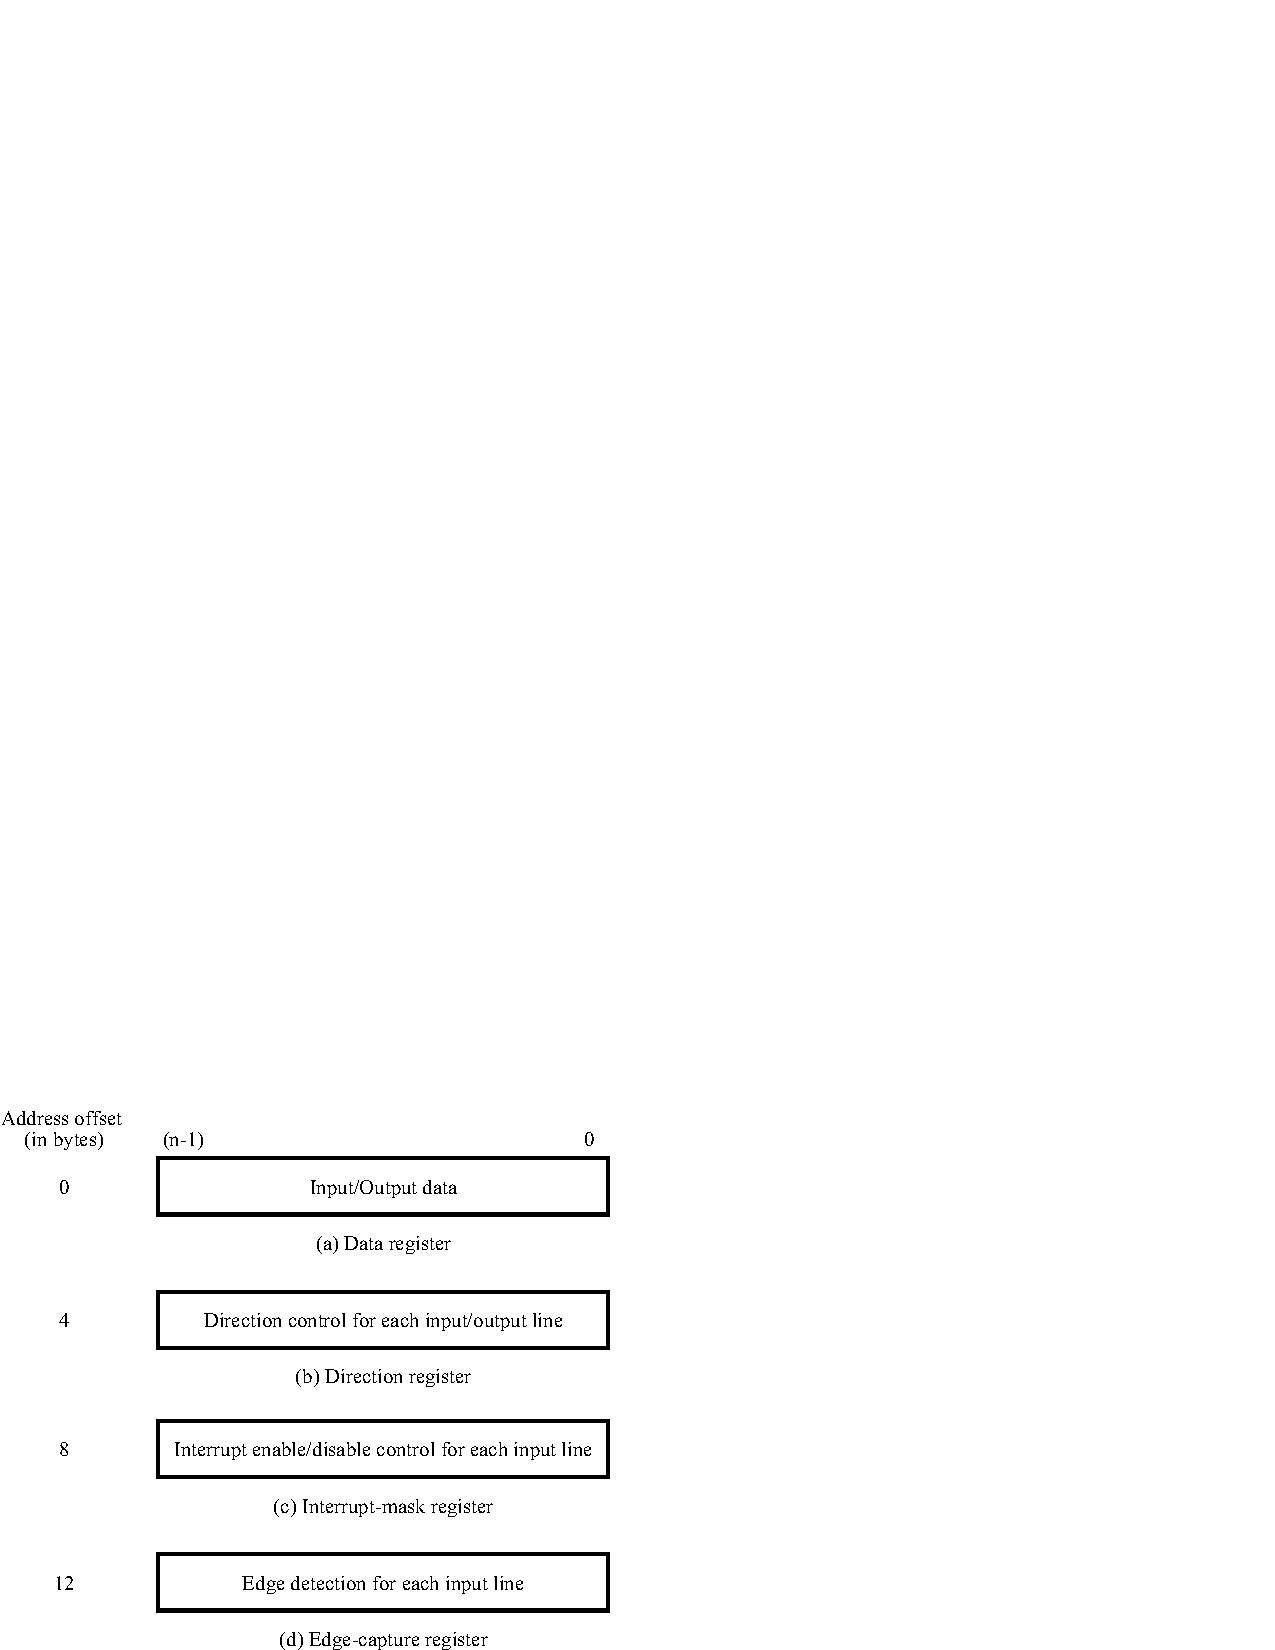
\includegraphics[scale=1]{figures/figureparallel.pdf}
	\end{center}
	\caption{Registers in the parallel port interface.}
\label{fig:parallel}
\end{figure}


Each register is $n$ bits long. The registers have the following purpose:
\begin{itemize}
\item {\it Data} register: holds the $n$ bits of data that are transferred between the parallel 
port and the Nios~II processor. It can be implemented as an input, 
output, or a bidirectional register.  \item {\it Direction} register defines the direction 
 of transfer for each of the $n$ data bits when a bidirectional interface is generated.
\item {\it Interrupt-mask} register: used to enable interrupts from the
input lines connected to the parallel port.
\item {\it Edge-capture} register: indicates when a change of logic value is detected in 
the signals on the input lines connected to the parallel port. Once a bit in the edge
capture register becomes asserted, it will remain asserted. An edge-capture bit can be
de-asserted by writing to it using the Nios~II processor.
\end{itemize}

Not all of these registers are present in some parallel ports. For example,
the {\it Direction} register is included only when a bidirectional interface is specified.
The {\it Interrupt-mask} and {\it Edge-capture} registers must be included if
interrupt-driven input/output is used.

~\\
The parallel port registers are memory mapped, starting at a specific {\it base} address.
The base address has to be a multiple of four if the parallel port is to be accessed using
word accesses from the Nios~II processor. The base address becomes the address of the {\it Data} 
register in the parallel port. The addresses of the other three registers have offsets 
of 4, 8, or 12 bytes (1, 2, or 3 words) from this base address.
The pre-built computer system all have parallel ports connected to slider switches, pushbutton KEYs, 
LEDs, and seven-segment displays (when those peripherals exist).

\section*{Part I}
\addcontentsline{toc}{1}{Part I}
Write a Nios~II assembly-language program that displays a decimal digit on the seven-segment
display {\it HEX}0. The other seven-segment 
displays on your DE-series board should be blank.  

~\\
The parallel port connected to the 
seven-segment displays {\it HEX}$3-0$ is memory mapped at the address {\sf 0xFF200020}, 
and the port connected to {\it HEX}$5-4$ is at the address {\sf 0xFF200030}.
Figure~\ref{fig:HEX} shows how the display segments are connected to the parallel ports.  

\begin{figure}[H]
	\begin{center}
	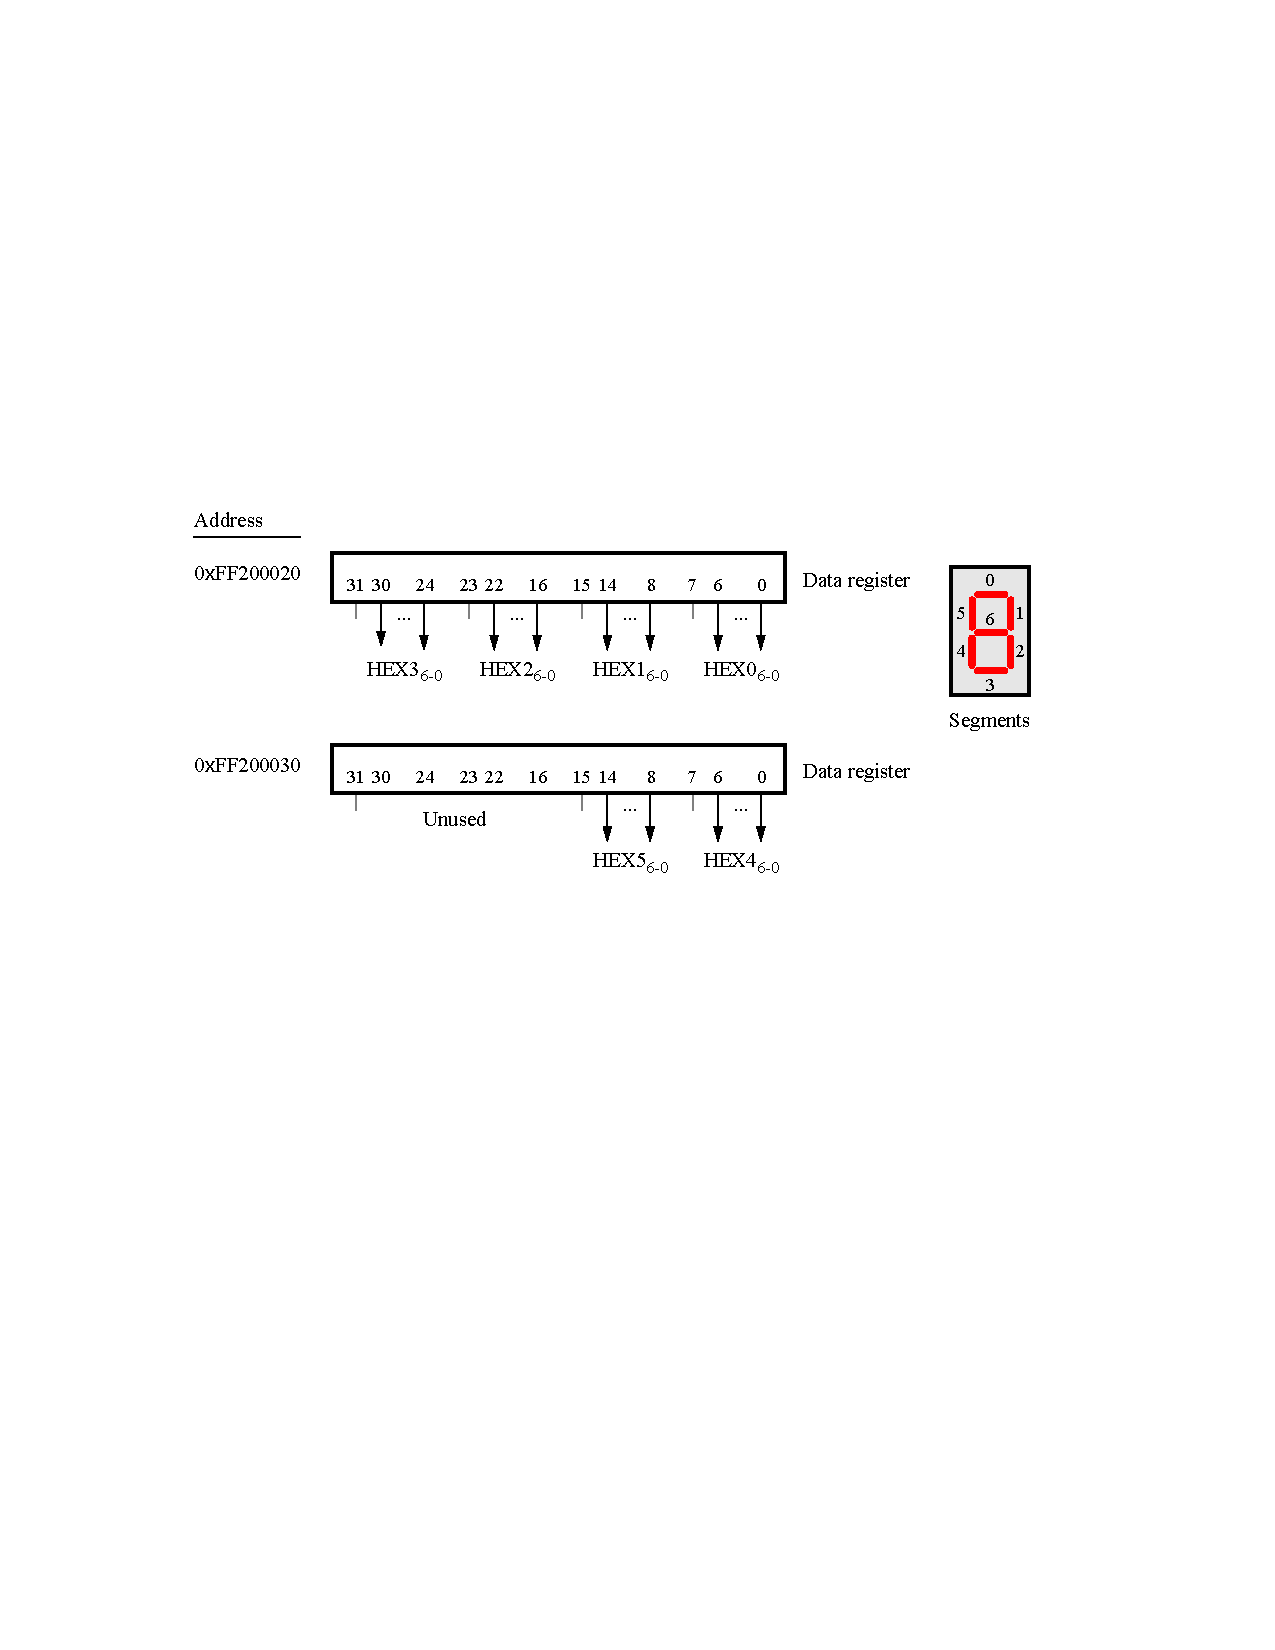
\includegraphics[scale=1]{figures/figureHEX.pdf}
	\end{center}
	\caption{The parallel ports connected to the seven-segment displays, {\it HEX}$5-0$, in the DE-series copmuter systems.}
\label{fig:HEX}
\end{figure}

Initially the number displayed on {\it HEX}0 should be 0.  If {\it KEY}$_1$ is pressed then {\it SW}$_0$ 
should be checked. If {\it SW}$_0$ is high increment the displayed number, and 
if it is low then decrement the number. Pressing {\it KEY}$_0$ should 
blank the display, and pressing any other KEY after that should return the display to 0.
The parallel port connected to the pushbutton {\it KEYs} is illustrated in Figure~\ref{fig:KEY}. 
The parallel port connected to the slider switches {\it SWs} is illustrated in Figure~\ref{fig:SW}. 
In your program, use polled I/O 
to read the {\it Data} register to see when a button is being pressed. When you are not pressing 
any {\it KEY} the {\it Data} register provides~0, and when you press {\it KEY}$_i$ the 
{\it Data} register provides the value 1 in bit position $i$. Once a button-press is detected,
be sure that your program waits until the button is released. You should not use the 
{\it Interruptmask} or {\it Edgecapture} registers for this part of the exercise.

\begin{figure}[H]
	\begin{center}
	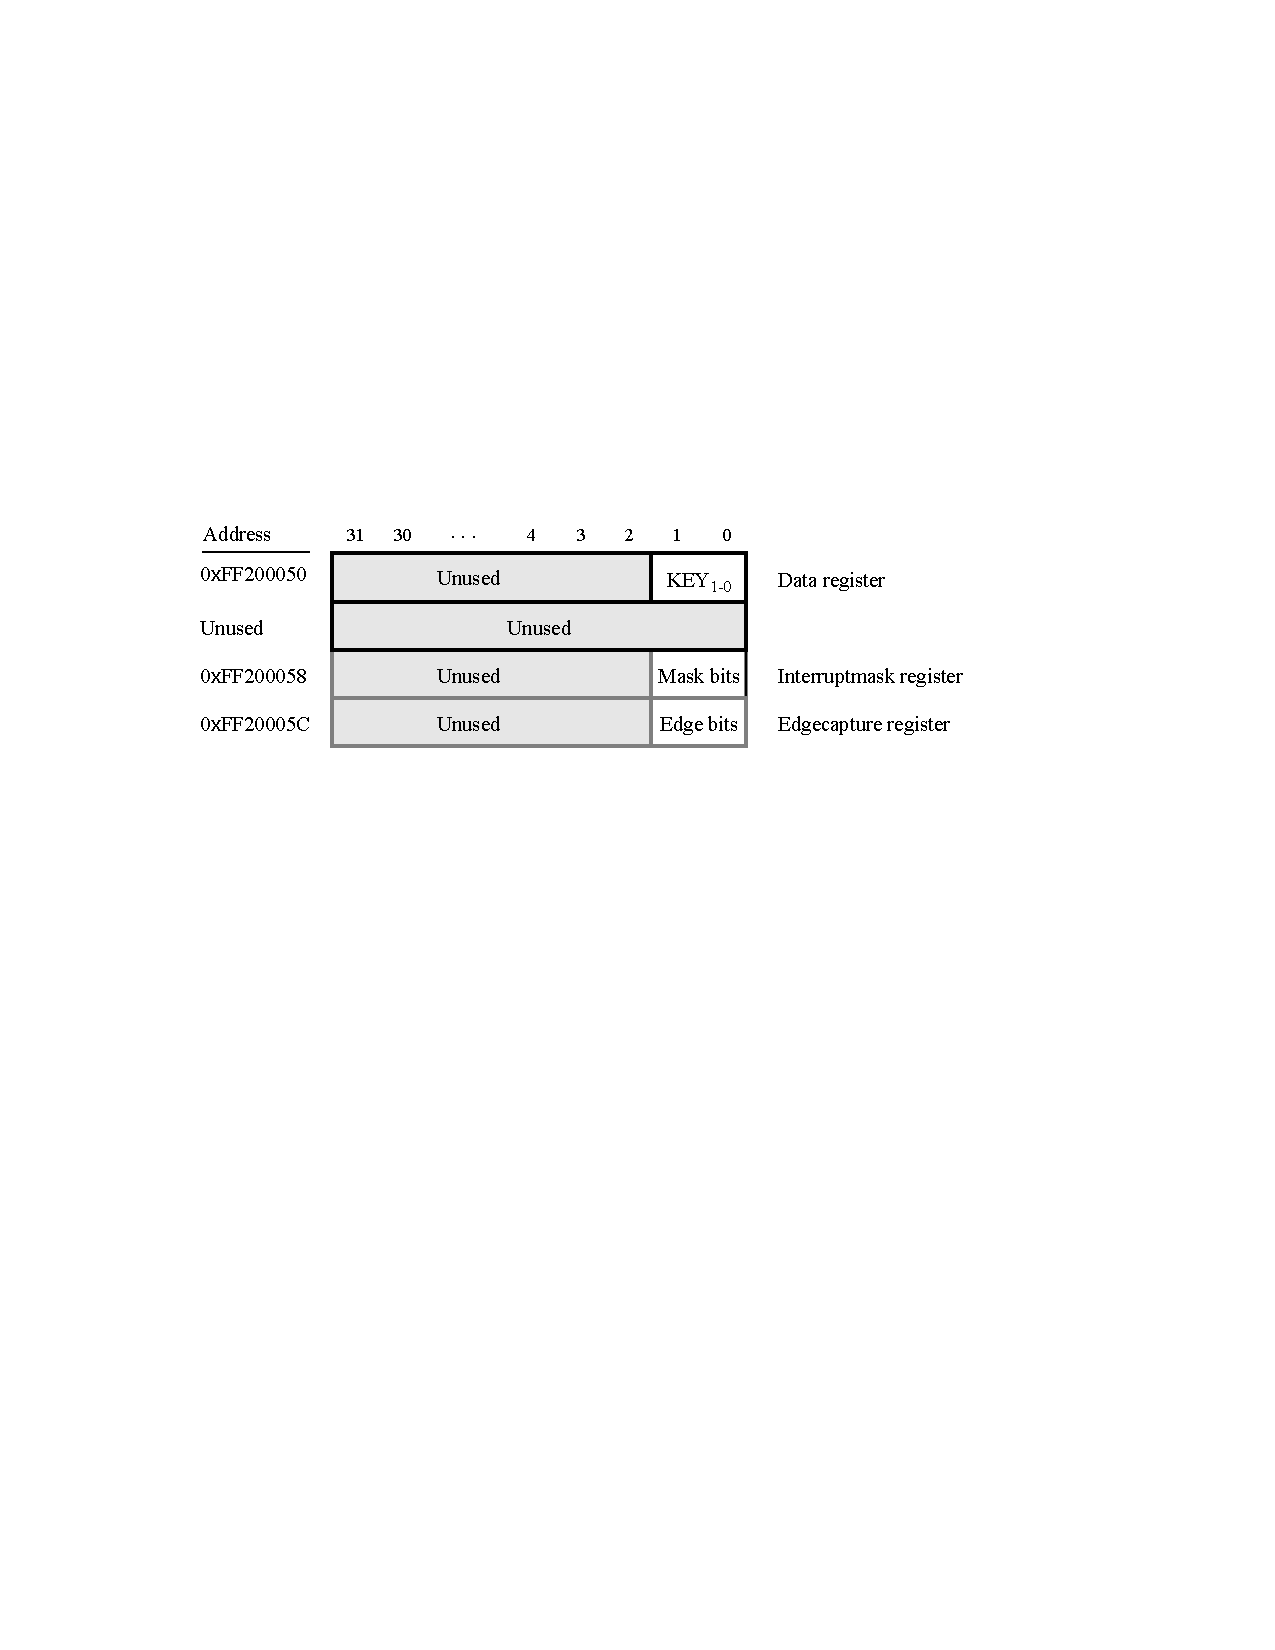
\includegraphics[scale=.9]{figures/figureKEY.pdf}
	\end{center}
	\caption{The parallel port connected to the pushbutton {\it KEYs}.}
\label{fig:KEY}
\end{figure}

\begin{figure}[H]
	\begin{center}
	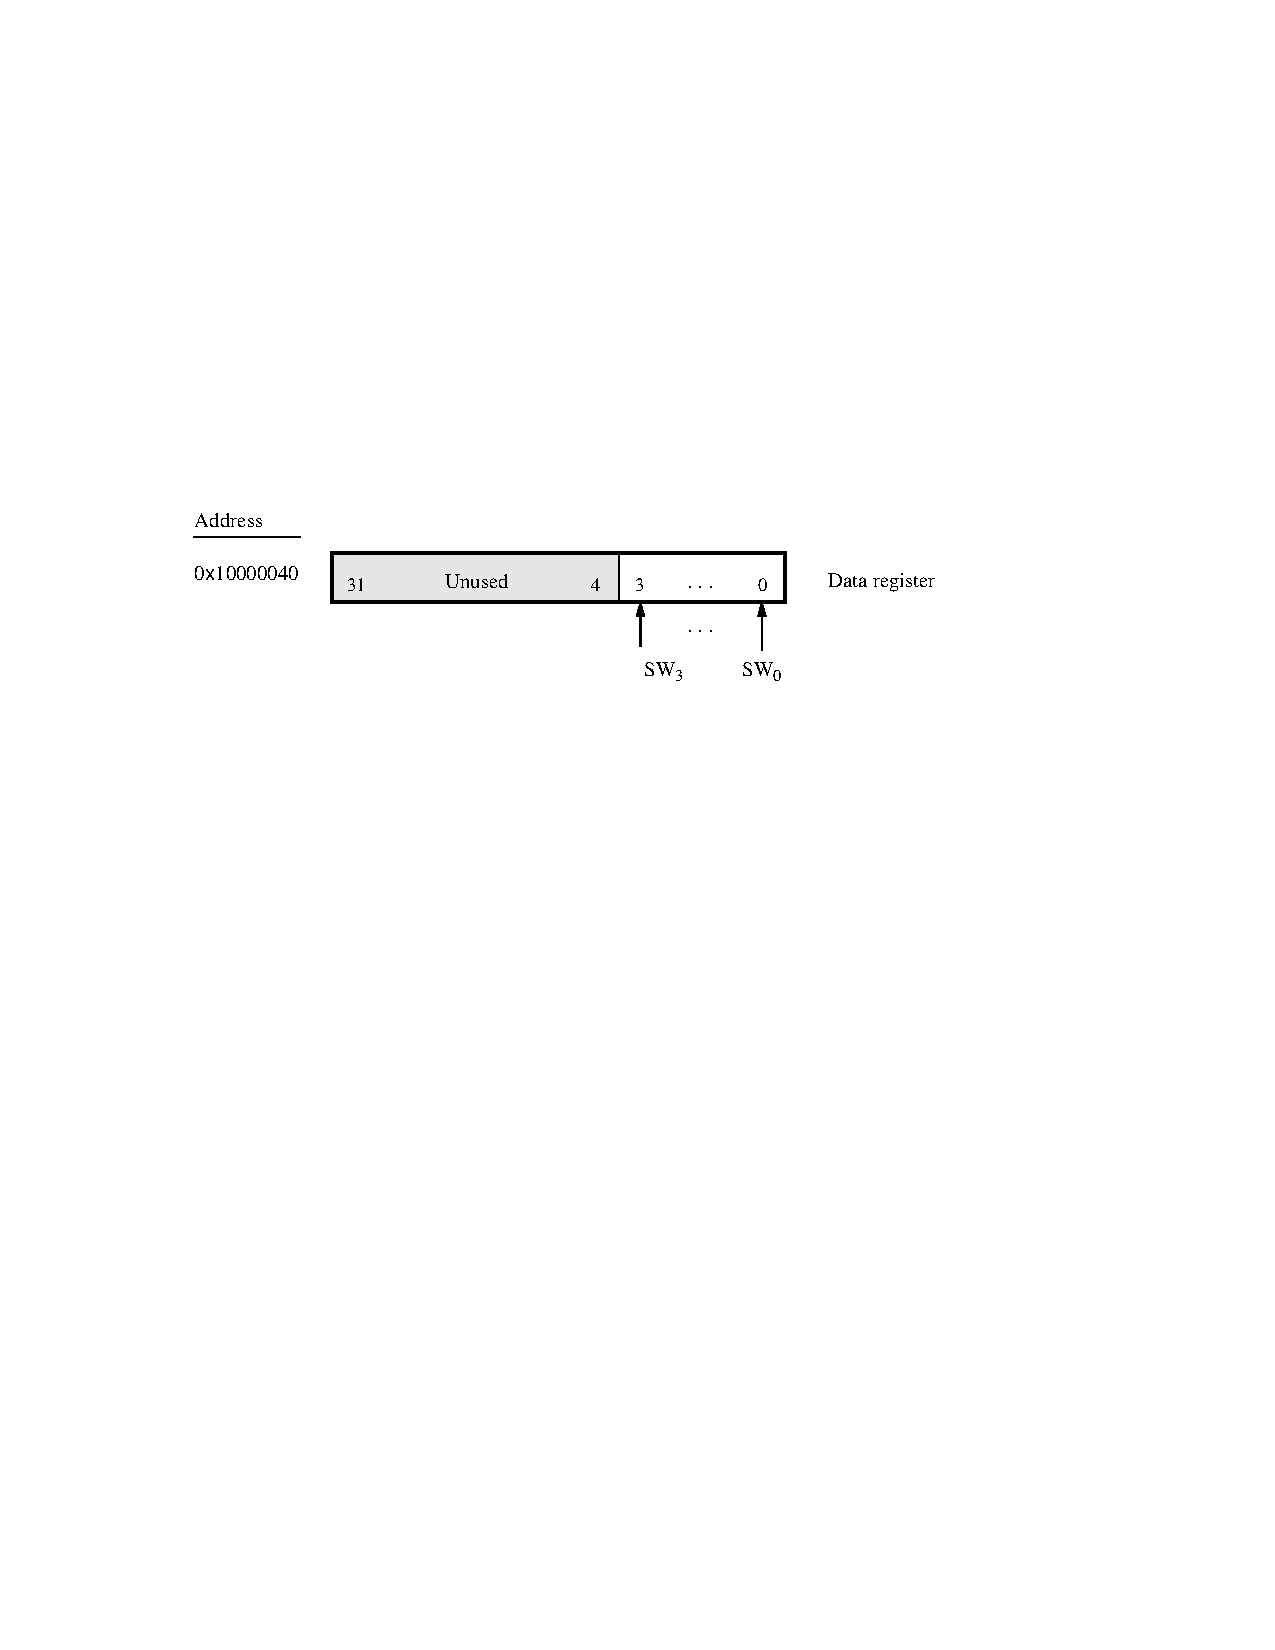
\includegraphics[scale=.9]{figures/figureSW.pdf}
	\end{center}
	\caption{The parallel port connected to the slider switches {\it SWs}.}
\label{fig:SW}
\end{figure}

Perform the following:

\begin{enumerate}
\item Create a new folder to hold your Monitor Program project for this part. Create a
file called {\it part1.s} and type your assembly language code into this file.
You may want to refer to a discussion, and examples of assembly-language code,
in Part IV of Lab Exercise 2 about displaying numbers on seven-segment displays.

\item
Make a new Monitor Program project in the folder where you stored the {\it part1.s} file.
Select Nios~II as the target processor architecture and use the appropriate pre-built 
computer system for your DE-series board.

\item
Compile, download, and test your program. 
\end{enumerate}

\section*{Part II}
\addcontentsline{toc}{2}{Part II}
Write a Nios~II assembly-language program that displays a two-digit decimal counter on the 
seven-segment displays {\it HEX}$1-0$. The counter should be incremented approximately
every $0.25$ seconds. When the counter reaches the value 99, it should start again at 0.
The counter should stop/start when any pushbutton {\it KEY} is pressed.

~\\
To achieve a delay of approximately 0.25 seconds, use a delay-loop in your assembly language
code. A suitable example of such a loop is shown below.

~\\
\begin{lstlisting}[style=defaultNiosStyle]
DO_DELAY: 	movia 	r7, 8000000 		# delay counter
SUB_LOOP: 	subi 	r7, r7, 1
			bne 	r7, zero, SUB_LOOP
\end{lstlisting}

~\\
To avoid ``missing'' any button presses while the processor is executing the delay loop, you
should use the {\it Edgecapture} register in the {\it KEY} port, shown in Figure~\ref{fig:KEY}.
When a pushbutton is pressed, the corresponding bit in the {\it Edgecapture} register is
set to 1, and it remains set until reset to 0 by writing into the register.


Perform the following:

\begin{enumerate}
\item Create a new folder to hold your Monitor Program project for this part. Create a
file called {\it part2.s} and type your assembly language code into this file.

\item
Make a new Monitor Program project in the folder where you stored the {\it part2.s}
file. Select Nios~II as the target processor architecture and use the appropriate pre-built 
computer system for your DE-series board.

\item
Compile, download, and test your program. 
\end{enumerate}

\section*{Part III}
\addcontentsline{toc}{3}{Part III}
In Part II you used a delay loop to cause the Nios~II processor to wait for approximately 0.25 
seconds. The processor loaded a large value into a register before the loop, and then 
decremented that value until it reached 0.  In this part you are to modify your code so that a
hardware timer is used to measure an exact delay of 0.25 seconds. You should use polled I/O to
cause the Nios~II processor to wait for the timer.

~\\
The pre-built computer systems include an {\it Interval Timer} implemented in the FPGA that can be used by
the Nios~II processor. This timer can be loaded with a preset value, and then counts down to 
zero using the 100-MHz clock signal provided as the system clock in the DE-series computer systems (or 50-Mhz for the DE2-115 Computer System). The programming interface 
for the timer includes six 16-bit registers, as illustrated in Figure~\ref{fig:timer}.

\begin{figure}[H]
	\begin{center}
	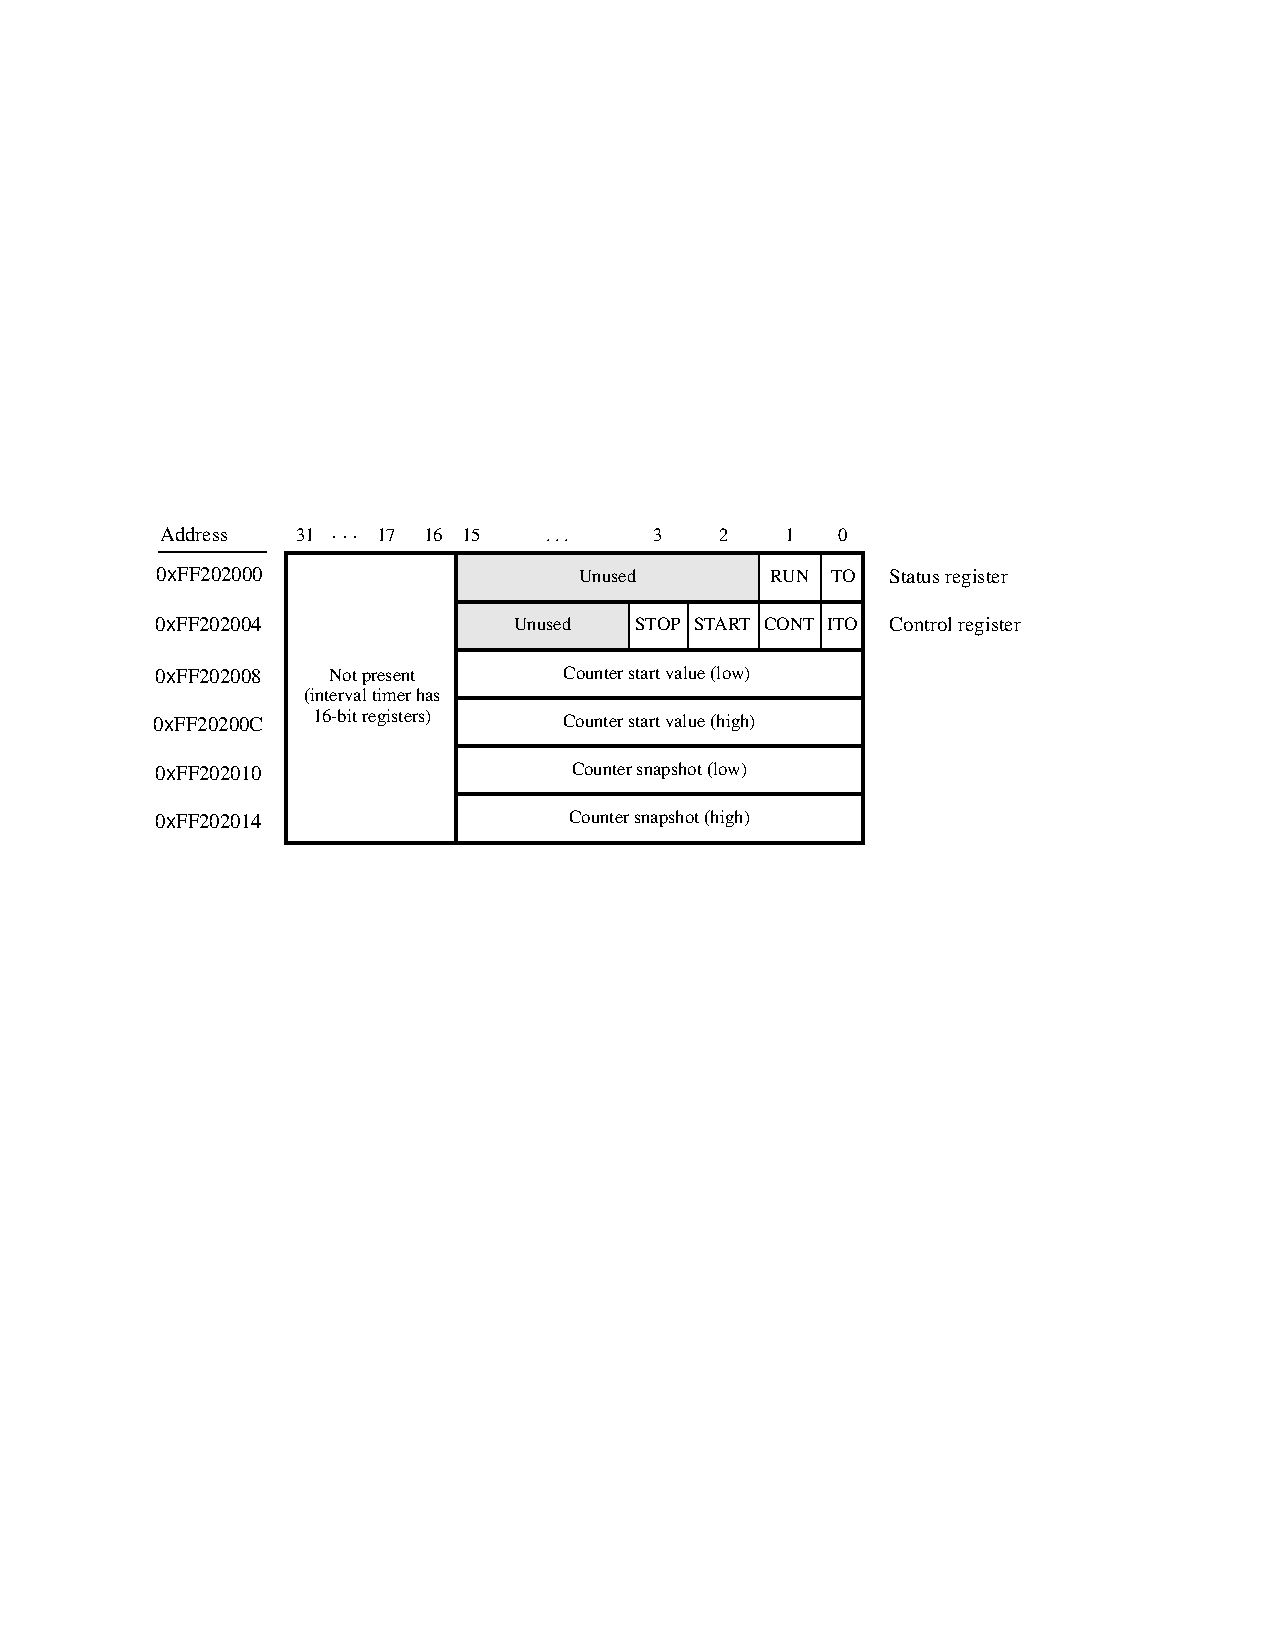
\includegraphics[scale=1]{figures/figuretimer.pdf}
	\end{center}
	\caption{The Interval Timer registers.}
\label{fig:timer}
\end{figure}

The {\it TO} bit in the {\it Status} register provides a timeout signal which is set to 1 
by the timer when it has reached a count value of zero.  
You should poll this bit in your program to cause the Nios~II processor 
to wait for the timer.  The {\it TO} bit can be reset by writing a 0 into it.  

~\\
The {\it CONT} bit affects the continuous operation of the timer.  When the timer reaches
a count value of zero it automatically reloads the specified starting count value. If 
{\it CONT} is set to 1, then the timer will continue counting down automatically.
But if {\it CONT} $=0$, then the timer will stop after it has reached a count value of 0. 
The ({\it START}/{\it STOP}) bits can be used to commence/suspend the operation of the 
timer by writing a 1 into the respective bit.

~\\
The two 16-bit registers for the Counter start value allow the period of the timer to be changed.
The default setting provided gives a timer period of 125 msec. To achieve this period, the starting value of the count is
100 MHz $\times$ 125 msec $=12.5\times10^6$.

~\\
Make a new folder to hold your Monitor Program project for this part. Create a
file called {\it part3.s} and type your assembly language code into this file.
Make a new Monitor Program project for this part of the exercise, and then compile, download, 
and test your program. 

\section*{Part IV}
\addcontentsline{toc}{4}{Part IV}
In this part you are to write an assembly language program that implements a real-time clock. 
Display the time on the seven-segment displays {\it HEX}$3-0$ in the format 
\red{SS}:\red{DD}, where \red{\it SS} are seconds and \red{\it DD} are hundredths of a second.
Measure time intervals of 0.01 seconds in your program by using polled I/O with the
Interval Timer.  You should be able to stop/run the clock by pressing any pushbutton {\it KEY}.
When the clock reaches \red{59}:\red{99}, it should wrap around to \red{00}:\red{00}.

~\\
Make a new folder to hold your Monitor Program project for this part. Create a
file called {\it part4.s} and type your code into this file.  Make a new Monitor Program 
project for this part of the exercise, and then compile, download, and test your program. 


%%%%%%%%%%%%%%%%%%%%%%%%%%%%%%%%%%%%%%%%
%%% FPGAcademy Copyright Information %%%
%%%%%%%%%%%%%%%%%%%%%%%%%%%%%%%%%%%%%%%%

%Always put the copyright on a new page (clear page), with some vertical space from top
\clearpage
\vspace{1in}

\noindent

Copyright {\copyright} FPGAcademy.org. All rights reserved. FPGAcademy and the 
FPGAcademy logo are trademarks of FPGAcademy.org.  This document is provided 
"as is", without warranty of any kind, express or implied, including but not 
limited to the warranties of merchantability, fitness for a particular purpose 
and noninfringement. In no event shall the authors or copyright holders be 
liable for any claim, damages or other liability, whether in an action of 
contract, tort or otherwise, arising from, out of or in connection with the 
document or the use or other dealings in the document.
~\\
~\\
**Other names and brands may be claimed as the property of others.


\end{document}
